% This text is proprietary.
% It's a part of presentation made by myself.
% It may not used commercial.
% The noncommercial use such as private and study is free
% Nov. 2006
% Author: Sascha Frank 
% University Freiburg 
% www.informatik.uni-freiburg.de/~frank/
%
% additional usepackage{beamerthemeshadow} is used
%  
%  \beamersetuncovermixins{\opaqueness<1>{25}}{\opaqueness<2->{15}}
%  with this the elements which were coming soon were only hinted

\documentclass{beamer}
\usepackage{listings}
\usetheme{Madrid}
\setbeamertemplate{items}[rectangle] 
\begin{document}
\title{Linux + Python}  
\author{Le\^onidas S. Barbosa}
\institute{
  Linux Technology Center - IBM \\
  \texttt{leosilva@linux.vnet.ibm.com}
}

\date[Setembro 2013]{12 de Setrembro, 2013} 

\frame{\titlepage} 

%\frame{\frametitle{Sum\'ario}tableofcontents} 
\begin{frame}{Sum\'ario}
 
\begin{itemize}
  \item Linux
  \item Python
\end{itemize}

\end{frame}

\begin{frame}
 
\center{Qual a resposta pra vida, o universo e tudo mais?}

\end{frame}

\begin{frame}
\center{42}
\begin{center}

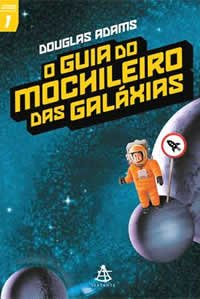
\includegraphics[width=0.2\textwidth]{images/guia.jpg} 
\end{center}
\end{frame}

\begin{frame}
 \center{http://pages.hacktoon.com/guia-programador-galaxias/}
 
\end{frame}


\begin{frame}
 
\center{Qual a resposta para a divers\~ao de um Hack/er/Nerd?}

\end{frame}

\begin{frame}

\center{Linux+Opensource Universe} 
\begin{center}
 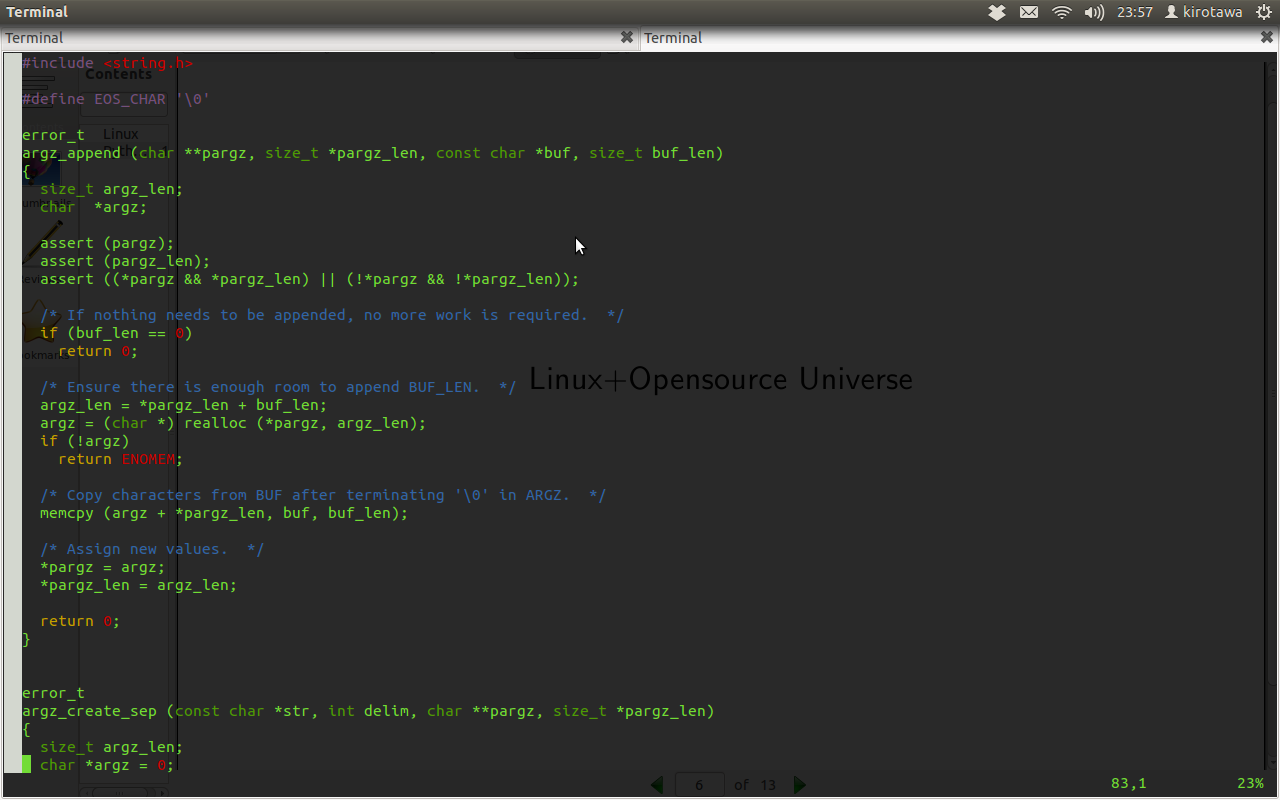
\includegraphics[width=0.9\textwidth]{images/opensource.png}
\end{center}
\end{frame}


\section{Linux} 
\frame{\frametitle{Linux} 
\begin{itemize}
 \item O que \'e Linux?
 \item Por que usar/investir em Linux?
 \item Quem usa Linux?
 \item Onde est\'a o Linux?
 \item Oportunidades com o Linux
\end{itemize}
}

\begin{frame}{O que \'e Linux?}

\begin{center}
 O kernel e ao mesmo tempo o SO que roda.
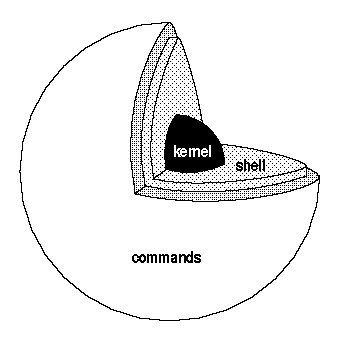
\includegraphics[width=0.5\textwidth]{images/kernel.jpg}
\end{center}

\end{frame}

\begin{frame}{Hist\'oria do Linux}
\begin{itemize}
  \item Minix
  \item Projeto GNU
  \item Mascote (tux)
\end{itemize}
 
\end{frame}

\begin{frame}{Hist\'oria do Linux}
\begin{center}
 
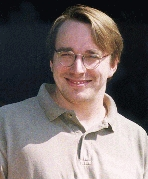
\includegraphics[width=0.3\textwidth]{images/liunus.jpg}
\center{Linus Torvalds}
\end{center}
\end{frame}

\begin{frame}{Hist\'oria do Linux}
 \begin{center}
  
\includegraphics[width=0.3\textwidth]{images/Gnulinux.png}
 \end{center}

 \center{Projeto GNU/Linux}

\end{frame}

\begin{frame}{Por que usar/investir em Linux?}
 
\begin{itemize}
 \item Seguro, robusto, divertido, configur\'avel, v\'arias distros...
 \item Mercado de Linux cresceu 80\% nos \'ultimos anos.
 \item Falta m\~ao de obra qualificada em Linux.
 \item Grandes empresas financiam e colaboram com o desenvolvimento do Linux.
\end{itemize}

\end{frame}

\begin{frame}{Quem usa Linux?}
\begin{itemize}
 \item Grandes centros de pesquisa: NASA, CERN, etc.
 \item Grandes empresas: Facebook, Google, IBM, Oracle, Microsoft (sim eles usam!), etc.
\end{itemize}

\end{frame}

\begin{frame}{Onde est\'a o Linux?}
\begin{itemize}
 \item Celulares
 \item Dispositivos embarcados
 \item Bancos, servidores, etc.
\end{itemize}

\end{frame}

\begin{frame}{Oportunidades com o Linux}

\begin{itemize}
 \item Grandes empresas e seus laborat\'orios: IBM, Intel, Microsoft, Google, Facebook, etc.
 \item Linux Technology Center - LTC - IBM (Hortol\^andia)
\end{itemize}
 

\end{frame}

\begin{frame}
 
Vagas no LTC :) 


Requisitos:
Formação em Ci\^encia ou Engenharia de Computa\c{c}\~ao ou \'areas correlatas;
Perfil desenvolvedor: design e implementa\c{c}\~ao em linguagens como C, Python ou Java;
Conhecimento sobre o uso de ferramentas de controle de versão como SVN ou Git;
Conhecimento sobre Arquitetura e Organiza\c{c}\~ao de Computadores, Sistemas Operacionais e Algoritmos;
Conhecimentos de uso e administra\c{c}\~ao em Linux \-\- Shell Scripts, administra\c{c}\~ao de pacotes, uso do Linux como Desktop no dia a dia;
Ingl\^es intermedi\'ario.


Diferenciais:
Ingl\^es avan\c{c}ado;
Participa\c{c}\~ao em comunidades Open Source: uso de listas de e-mail e patches, GNU Toolchain (gcc, gdb), GNU autotools e esquemas de empacotamento como RPM ou Debian;
Conhecimento sobre metodologias \'Ageis de desenvolvimento de software.


Para se candidatar, basta acessar o sistema de vagas da IBM através do site http://www.ibm.com/br/employment  e buscar pelo c\'odigo da vaga:
Profissionais com Gradua\c{c}\~ao completa a partir de Janeiro de 2012 ou a completar at\'e Dezembro de 2013: c\'odigo STG-0601560
Profissionais com Mestrado completo a partir de Janeiro de 2012 ou a completar at\'e Dezembro de 2013: c\'odigo STG-0601532
\end{frame}

\begin{frame}
\begin{center}
   
\includegraphics[width=0.3\textwidth]{images/tux.jpg}
\end{center}
\end{frame}


\section{Python}
\frame{\frametitle{Python} 
 \begin{itemize}
  \item O que \'e?
  \item Como surgiu?
 \end{itemize}
}

\begin{frame}{O que \'e?}
 \begin{itemize}
  \item Linguagem de Alto n\'ivel
  \item Dinamicamente tipada e de tipagem forte
  \item Interpretada
  \item Imperativa, funcional e orientada a objetos
  \item Implementada em C (CPython)
  \item Linguagem de prop\'osito geral
 \end{itemize}

\end{frame}

\begin{frame}{Como surgiu?}
 \begin{itemize}
  \item Guido van Rossum
   
 \end{itemize}

\end{frame}

\begin{frame}{Come\c{c}ando com Python}
 \begin{itemize}
  \item Shell interativo
  \item Fun\c{c}\~ao help()
  \item M\'etodo \_\_doc\_\_
  \item Fun\c{c}\~ao dir()
 \end{itemize}

\end{frame}


\begin{frame}{Hello World!}
\begin{Example}
print ``hello World''
\end{Example}

\end{frame}

\begin{frame}{Sintaxe}
 \begin{itemize}
  \item Indenta\c{c}\~ao obrigat\'oria
  \item Padr\~ao, PEP08
 \end{itemize}

\end{frame}

\begin{frame}{IO - Entrada e sa\'ida}
 \begin{itemize}
  \item print
  \item raw\_input, input
 \end{itemize}

\end{frame}

\begin{frame}{IO - Entrada e sa\'ida}
\begin{Example}
  raw\_input(``Digite o seu nome'')
\end{Example}

\begin{Example}
input(``Digite sua idade'')
\end{Example}

\end{frame}

\begin{frame}{Codifica\c{c}\~ao e execu\c{c}\~ao}
 
 \begin{itemize}
  \item Execu\c{c}\~ao: arquivo.py
  \item Codifica\c{c}\~ao : unicode/utf-8, etc.
 \end{itemize}
 
 \begin{Example}
  \#!/usr/bin/env/python
 \end{Example}
\begin{Example}
 \# -*- coding: utf-8 -*-
\end{Example}


\end{frame}

\begin{frame}{Exemplo de c\'odigo em Python}
 \begin{center}
   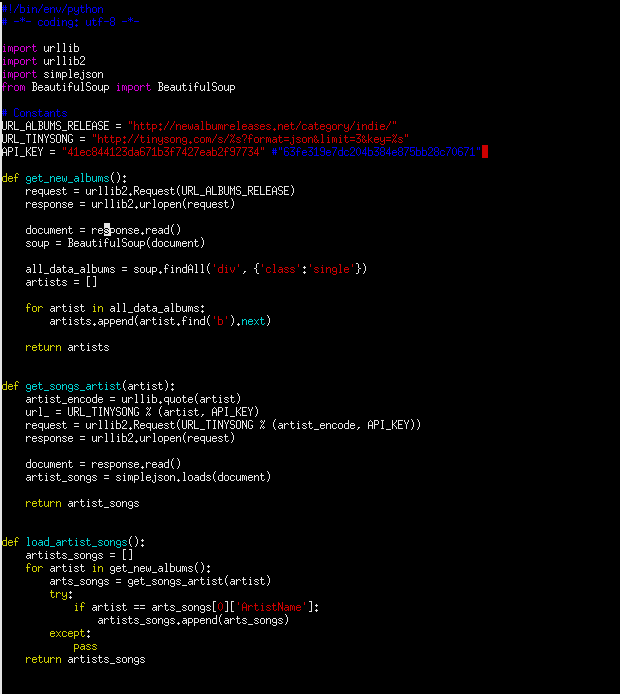
\includegraphics[width=0.5\textwidth]{images/code_py.png}
\end{center}
\end{frame}

\begin{frame}{Tipos e tipagem din\^amica}
 \begin{itemize}
  \item str, int, float, complexo, booleano, None
 \end{itemize}
 
 \begin{center}
   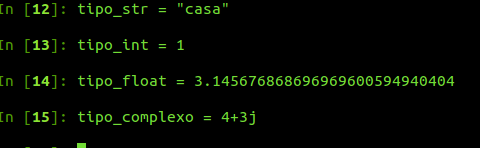
\includegraphics[width=0.5\textwidth]{images/tipos_py.png}
\end{center}

\end{frame}

\begin{frame}{Tudo \'e Objeto}
 \begin{itemize}
  \item str
  \item int
  \item float
  \item booleano
  \item None
 \end{itemize}

 \begin{center}
   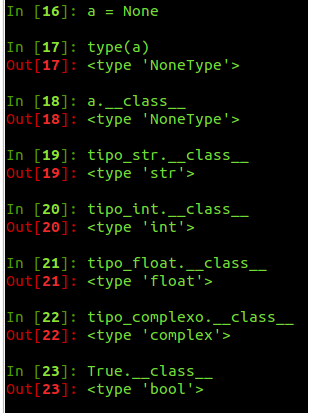
\includegraphics[width=0.3\textwidth]{images/quasetudo_objeto.png}
\end{center}
\end{frame}

\begin{frame}{Vamos explorar!}
 \begin{itemize}
  \item Usando o shell do python criem vari\'aveis com nome qualquer. Atribuam a ela o tipo que voc\^es quiserem. 
  \item Agora atribua outro tipo a mesma vari\'avel. 
   \item Use type(var\_name) e veja o que aconteceu.
 \end{itemize}

\end{frame}

\begin{frame}{Explorando...}
 \begin{itemize}
  \item Crie agora um arquivo .py
  \item Crie uma vari\'avel str e atribua a frase: ``N\~ao entre em p\^anico''
  \item Salve e execute python arquivo.py
  \item O que aconteceu? Algum erro? Como consert\'a\--lo

 \end{itemize}

\end{frame}

\begin{frame}{Controle de Fluxo}
  \begin{center}
   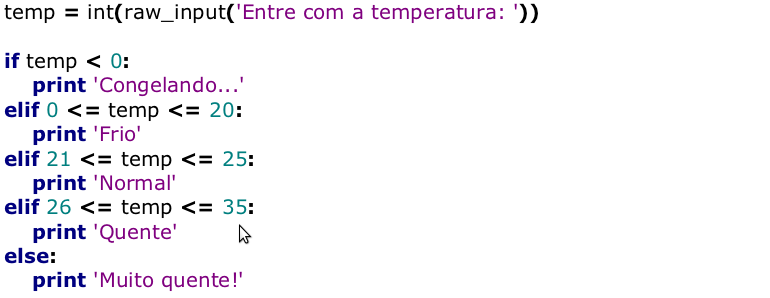
\includegraphics[width=0.5\textwidth]{images/controle_fluxo.png}
\end{center}
 \begin{center}
   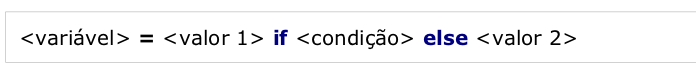
\includegraphics[width=0.5\textwidth]{images/ternario.png}
\end{center}
\end{frame}

\begin{frame}{Vamos explorar!}
 \begin{itemize}
  \item Utilizando apenas ifs e elses, crie um script em Python que leia do teclado 3 n\'umeros e retorne o maior deles.
  \item Em python '\%' \'e o operador de modulo, retornando o resto da divis\~ao de dois n\'umeros. Crie um script Python que receba 5 n\'umeros quaisquer e ao final retorne apenas os n\'umeros impares, se houver algum.
 \end{itemize}

\end{frame}

\begin{frame}{Operadores matem\'aticos}
 \begin{itemize}
  \item +,-, *, **, \%, / e //
 \end{itemize}

\end{frame}

\begin{frame}{Explorando...}
 \begin{itemize}
  \item Somar, subtrair e multiplicar todos sabem, mas e o uso de / e //, dividir? Qual a diferen\c{c}a, vamos tentar descobrir. Nota: A divis\~ao de floats requer que voc\^e acrescente ponto ao n\'umero, por exemplo 3 / 2.0, retornar\'a um float como resultado.
  \item O que acontece se voc\^e multiplicar uma palavra ``casa'' * 3 ?
 \end{itemize}

\end{frame}

\begin{frame}{La\c{c}os de repeti\c{c}\~ao}
 \begin{itemize}
  \item for, while
  
  \begin{center}
   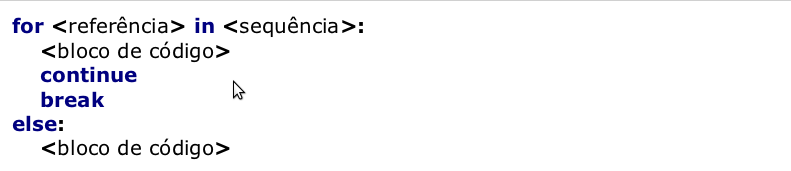
\includegraphics[width=0.5\textwidth]{images/for.png}
\end{center}
\begin{center}
   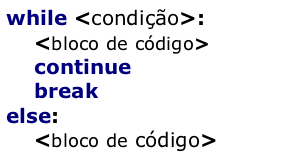
\includegraphics[width=0.5\textwidth]{images/while.png}
\end{center}
 \end{itemize}

\end{frame}

\begin{frame}{Explorando...}
 \begin{itemize}
  \item Vamos explorar o for. Crie um for de 1 at\'e 15, mas pulando de dois em dois n\'umeros. Exemplo: 1,4,7,10... Dica: use a fun\c{c}\~ao range() - Verifique com a fun\c{c}\~ao help como utiliz\'a\--la
  \item  Crie um script Python que receba n\'umeros do teclado e enquanto -1 n\~ao for dado como entrada ele fique rodando. Cuidado com o  loop infinito =P
 \end{itemize}

\end{frame}

\begin{frame}{Estruturas de Dados}
 \begin{itemize}
  \item listas
  \item tuplas
  \item dicion\'arios
 \end{itemize}

\end{frame}

\begin{frame}{Listas}
 \begin{center}
   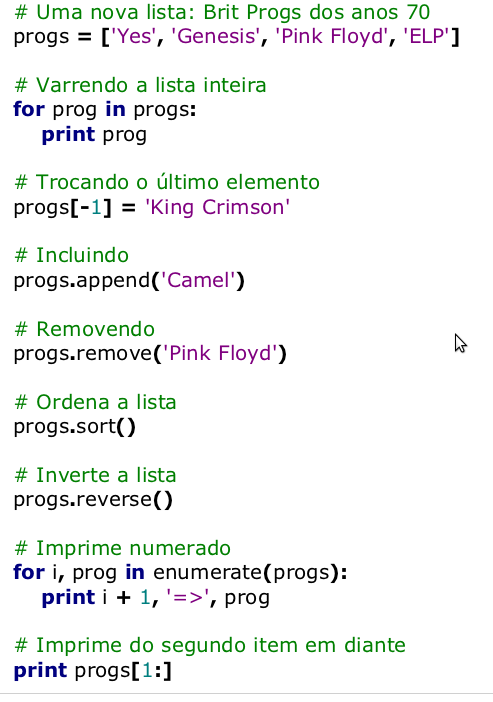
\includegraphics[width=0.3\textwidth]{images/listas.png}
\end{center}
 
\end{frame}
\begin{frame}{Slices}
 \begin{center}
   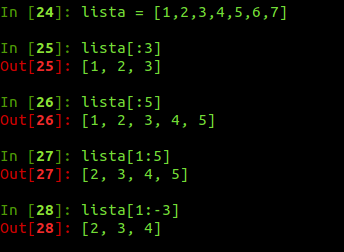
\includegraphics[width=0.5\textwidth]{images/slice.png}
\end{center}
\end{frame}

\begin{frame}{List Comprehensions}
 \begin{itemize}
  \item Um jeito conciso de criar listas
 \end{itemize}

 \begin{center}
   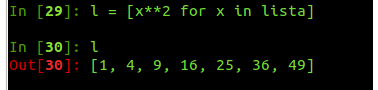
\includegraphics[width=0.5\textwidth]{images/comprehensions.png}
\end{center}
\end{frame}

\begin{frame}{Vamos explorar!}
 \begin{itemize}
  \item Conhecer os m\'etodos que uma lista possui
  \item Criar uma lista vazia
  \item Adicionar elementos a lista
  \item ordenar a lista
  \item Retornar o \'ultimo elemento da lista e o tamanho da lista
  \item Retornar a lista ao contr\'ario
  \item Contar a ocorr\^encia de um dado elemento na lista
  \item Usando um for incremente mais um a cada elemento da lista
  \item Crie uma lista usando list comprehensions que dada uma string gera uma lista dela e acrescente xpto como sufixo de cada palavra. Por fim
escreva a frase nova com a string manuseada.
 \end{itemize}

\end{frame}

\begin{frame}{Tuplas}
 \begin{itemize}
  \item Similar a listas. Por\'em imut\'avel.
  
 \end{itemize}

  \begin{center}
   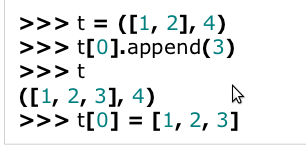
\includegraphics[width=0.5\textwidth]{images/tuplas.png}
\end{center}
\end{frame}

\begin{frame}{Explorando...}
 \begin{itemize}
  \item Vamos descobrir por que tuplas s\~ao imut\'aveis! Crie uma lista com 2 tuplas, cada tupla contendo respectivamente: 3 tuplas (coordenadas de um triangulo), 4 tuplas (coordenadas de um retangulo).
  \item Crie um programa que leia as coordenadas de cada tupla. Com um menu (ouch!) onde uma das op\c{c}\~oes \'e de modificar as coordenadas de um dado ponto. O que acontece?
 \end{itemize}

\end{frame}

\begin{frame}{Dicion\'arios}
 \begin{itemize}
  \item Dicion\'arios s\~ao nada mais  que hashes de acesso direto.
 \end{itemize}

  \begin{center}
   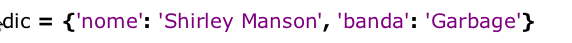
\includegraphics[width=0.5\textwidth]{images/dicionario.png}
\end{center}
\end{frame}

\begin{frame}{Explorando...}
 \begin{itemize}
  \item Crie um script Python que receba os dados do seus colegas do lado. Nome, Idade, Sexo, Curso. Armazene em uma lista de dicion\'arios. 
  \item Dado um nome busque na lista de dicionarios, caso encontre print os dados do colega na tela.
  
 \end{itemize}

\end{frame}

\begin{frame}{Operadores Booleanos}
  \begin{center}
   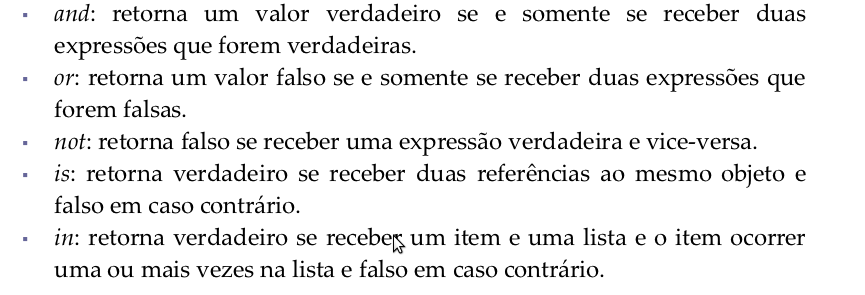
\includegraphics[width=0.7\textwidth]{images/booleanos.png}
\end{center}
\end{frame}

\begin{frame}{Desafios em Python}
\begin{itemize}
 \item http://www.pythonchallenge.com/
\end{itemize}

 
\end{frame}


\end{document}
